
\begin{figure}
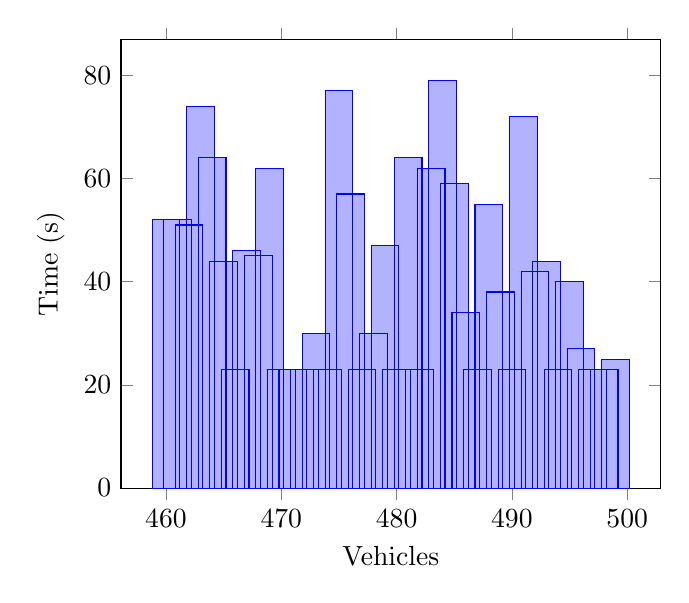
\begin{tikzpicture}
\begin{axis}[
legend style={anchor=west},
xlabel=Vehicles,
ylabel=Time (s),
ymin=0,
ybar,
]
\addplot coordinates {
(497, 23)
(499, 25)
(494, 23)
(495, 40)
(490, 23)
(491, 72)
(492, 42)
(493, 44)
(498, 23)
(464, 64)
(496, 27)
(469, 62)
(468, 45)
(465, 44)
(466, 23)
(461, 52)
(460, 52)
(463, 74)
(462, 51)
(467, 46)
(481, 64)
(489, 38)
(488, 55)
(487, 23)
(486, 34)
(485, 59)
(484, 79)
(483, 62)
(482, 23)
(480, 23)
(472, 23)
(473, 30)
(470, 23)
(471, 23)
(476, 57)
(477, 23)
(474, 23)
(475, 77)
(478, 30)
(479, 47)
};

\end{axis}
\end{tikzpicture}
\label{tik:time:100:79}
\caption{100 percent diving with GSC on route $79$}
\end{figure}
